%#!xelatex
\documentclass[b5paper,xelatex,ja=standard]{bxjsarticle} % 日本語用クラスファイル

\usepackage{showexpl}
\lstset{pos=l, width=.4\textwidth,
  explpreset={numbers=left,numberstyle=\tiny,literate={\\\\}{}0 }}
% showexplの出力が邪魔なので表示しない
\makeatletter\let\SX@Info=\relax\makeatother

% 更新日時の印字に datetime2 パッケージの \DTMnow を使う
% ただし, datetime2 パッケージは \today を上書きしようとするので,防止する
% また,タイムゾーンは印字しない
\let\origtoday=\today
\usepackage[datesep={/},timesep={:}]{datetime2}
\renewcommand\DTMdisplayzone[2]{}
\let\today=\origtoday

\usepackage{mystyle}
\usepackage{pxrubrica} % should be loaded after xeCJK package

\usepackage{fontspec}
\usepackage{unicode-math}
% \newfontfamily\LatinModernMath{latinmodern-math.otf}
% \newfontfamily\STIXMath{STIXMath-Regular.otf}
\newfontfamily\FiraMath{FiraMath-Regular.otf}

\hypersetup{
  %pdfusetitle, % なぜか効かない
  pdftitle={pTeX系列以外による日本語文書作成},
  pdfkeywords={MiKTeX, pdfTeX, XeTeX, LuaTeX, BXcjkjatype, ZXjatype, LuaTeX-ja}
}
\title{\pTeX 系列以外による日本語文書作成}
\date{\today}
\author{}
\captionsetup{justification=centering, labelfont={small, rm}}

\begin{document}
\catcode`\<=13
\def<#1>{$\langle${\rmfamily\itshape#1}$\rangle$}

\maketitle

\footnotetext[0]{%
本文書は\XeTeX と\PKG{ZXjatype}パッケージを用いて組版した.
それ以外の「\TeX~Liveのインストール」「\TeX 実習」は,\LuaTeX-jaを
用いて組版している.
}

Knuth氏は,1990年にこれ以上\TeX\footnote{本文書では,
Knuth氏の作成した(プログラムとしての)\TeX を\emph{\TeX82}%
と呼ぶことにする.}の機能拡張を行わないことを宣言した:
\begin{quotation}
\rightskip3\jsZw\parindent2em

\noindent\indent
My work on developing \TeX, \MF, and Computer
Modern has come to an end. I will make no further
changes except to correct extremely serious bugs.

I have put these systems into the public domain so that
people everywhere can use the ideas freely if they wish.
$\ldots$\ Let us regard
these systems as fixed points, which should give
the same results 100 years from now that they produce
today.

\smallskip

\raggedleft  --- Donald~E. Knuth, \textit{The future of \TeX\ and \MF},
TUGboat~\emph{11}, No.~4,  1990.\\
\url{http://tug.org/TUGboat/Articles/tb11-4/tb30knut.pdf}
\end{quotation}

しかし,これで「\TeX は終わった」わけではない.上の引用の第2段落にあるとおり,
\TeX82を改良して(別の名前で\footnote{%
この「内容を改変した場合は別の名称にしなければならない」というのは
\TeX 業界での特徴的な約束事である.})公開することは自由であり,
今まで世界中で数々の拡張が試みられ,現在でも拡張の開発が進められている%
\footnote{日本で主流の\pTeX,またu\pTeX に関しても,バグ修正や不自然な挙動の改善が
  現在でも時々なされている.}.
詳しくは
\begin{itemize}
\item 八登崇之,「日本人の知らない\TeX---\TeX の過去・現在・未来」,
\TeX ユーザの集い2010.\\
\url{http://zrbabbler.sp.land.to/texconf10.html}
\item 寺田侑祐,「\href{https://www.slideshare.net/doraTeX/the-history-of-tex-and-its-recent-advances}{近年の\TeX の動向}」,
\href{http://www.mathlibre.org/msfd/18-ja.html}{数学ソフトウェアとフリードキュメントXVIII}.
\item Arno Trautmann, \textit{%
  An overview of \TeX, its children and their friends $\ldots$\,}\\
\url{http://mirrors.ctan.org/info/tex-overview/tex-overview.pdf}
\item \href{https://texwiki.texjp.org/}{\TeX~Wiki}\>
  中の「\LuaTeX」「\XeTeX」「\upTeX」「\eTeX」等の各記事
\end{itemize}
などを参照.

\medskip
\pTeX ももちろん\TeX82の拡張であるのだが,
本文章では,\emph{\pTeX 系列以外の代表的な\TeX82の拡張}と,
それによって日本語文書を作成する方法について述べる.
取り扱うのは表\>\ref{tab:non-ptex}\>に載せた3つの方法である\footnote{%
表\>\ref{tab:non-ptex}\>には比較のため,「\pTeX${}+{}$\DVIPDFMx」も載せている.}.

\begin{table}[ht]
\caption{本文書で扱う\pTeX 系列以外の\TeX}
\label{tab:non-ptex}\centering\small
\begin{tabular}{cccccr}
\toprule
\emph{節}&\emph{プログラム}&\emph{パッケージ}&\multicolumn{2}{c}{\emph{ドライバ指定}}&\\
\cmidrule(lr){4-5}
&&&\PKG{graphicx}&\PKG{hyperref}&\\
\midrule
\S\ref{sec:pdftex}
&\pdfTeX&\PKG{CJK}, \PKG{bxcjkjatype}&\texttt{pdftex}(自動)&\texttt{pdftex}(自動)\\
\S\ref{sec:xetex}
&\XeTeX&\PKG{xeCJK}, \PKG{zxjatype}&\texttt{xetex}(自動)&\texttt{xetex}(自動)\\
\S\ref{sec:luatex}
&\LuaTeX&\LuaTeX-ja&\texttt{pdftex}(自動)&\texttt{pdftex}(自動)\\
\midrule
(&\pTeX${}+{}$\DVIPDFMx&---&\texttt{dvipdfmx}&\texttt{dvipdfmx}&)\\
\bottomrule
\end{tabular}
\end{table}


\vfill

{\scriptsize\raggedleft
Last update: \texttt{\DTMnow}.
\par}

\newpage
\tableofcontents

\newpage

\section{導入}

「\TeX を使って日本語文書を作成する」と言った場合,
「\TeX 実習」で説明したように\pTeX ・u\pTeX を用いるのが一般的であろう.
受講生の中には,「\pTeX ・u\pTeX で十分.なぜ他の方法を気にするのか?」と
思う方もいるかもしれない.しかし,あくまで筆者の私見だが,以下の2つの
理由で重要である:
\begin{itemize}
 \item \emph{「\TeX が入っている」と「\pTeX が利用できる」とは同義ではない.}\\
\pTeX 自体は1990年代からあるが,それが「上流」の\TeX~Liveで利用できるようになったのは2010年という
比較的最近である.
また,すぐ後に述べるMiK\TeX という
Windows用の\TeX ディストリビューションでは,
\pTeX は未だに含まれていない.
 \item \emph{世界での\TeX の発展に\pTeX は取り残されている}\\
海外では,\pdfTeX~(\S\ref{sec:pdftex})などを利用したPDF直接生成が当たり前になっている.
さらには\XeTeX~(\S\ref{sec:xetex}), \LuaTeX~(\S\ref{sec:luatex})においては
Unicodeへの本格的な対応やOpenTypeフォントの機能が利用できるようになっている.

一方,\pTeX は大雑把に言えば「\TeX82を日本語拡張しただけ」である.
実際には\eTeX 拡張がサポート($\varepsilon$-p\TeX)されていたり,
u\pTeX で「和文の部分」がUnicode化されたりしているが,これ以上の機能拡張はもう
あまり行われないだろう.
\end{itemize}


例えば,\href{https://miktex.org/}{\emph{MiK\TeX}}\>という
海外でよく使われているWindows用の\TeX ディストリビューションがある.
面白いのは,MiK\TeX のパッケージとしては存在するが
システムにまだインストールされていないファイルがタイプセット時に
要求された場合,自動的に
\begin{center}
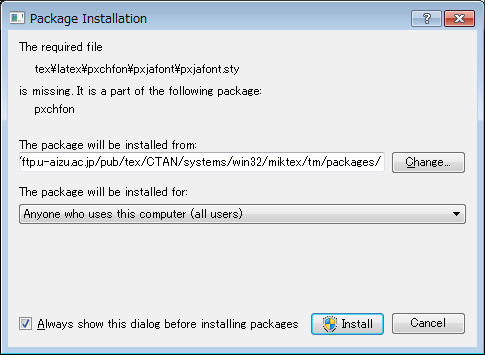
\includegraphics[scale=0.5]{mik-inst.png}
\end{center}
のようなダイアログが出て,インターネットから取得することができることである.


しかし,MiK\TeX には\pLaTeX が含まれていないので,日本語文書を
作りたい場合は,本文書の残りで説明するような別の方法を用いないといけない.
実は,本文書をつくるきっかけは,
数年前の\TeX 実習における受講生の「MiK\TeX で日本語文書は作成できないのか」
という質問であった.



\newpage

\section{予備知識:\eTeX 拡張}
\label{sec:etex}
表\>\ref{tab:non-ptex}\>に載せた4つのどの方法でも使えるのが,\emph{\eTeX 拡張}である.
これはThe \NTS{} team (Peter Breitenlohner et~al.)によって
開発された\TeX82の拡張であり,
一般利用者にとって特に有用なものを挙げると,次のようなものがある.
\begin{itemize}
\item \verb!\numexpr 4-(3*2)+\count0!のように内部整数・長さなどを
  式の形で表現できる.
\item 使用可能なレジスタが各種類ごとに256個から32768個まで激増した\footnote{%
  \LuaTeX{}ではさらに65536個まで増えている.}.

これにより,たくさんパッケージ読み込んだときに発生しうる
\begin{lstlisting}
! No room for a new \count .
\end{lstlisting}
がほとんど起こらなくなった.
% 実際には,このエラーはレジスタ確保用の\emph{マクロ}が出している.
% 以前は\LaTeX では\PKG{etex}パッケージを読み込むなどしてマクロ側で対応させる必要があったが,
% 最近(2015年以降?)は\LaTeX カーネル自身がe-TeX拡張を検出して対応するようになった.

\item 数式中の「サイズが自動的に変わる括弧」に使われる\verb+\left+・
  \verb+\right+に加えて,\verb+\middle+が利用できるようになった.
  例えば量子力学のDirac記法,例えば
\[
 \left\langle \phi \middle| \frac{\partial^2}{\partial t^2} \middle| \psi \right\rangle
\]
を,
\begin{lstlisting}
\left\langle \phi \middle| \frac{\partial^2}{\partial t^2}
  \middle| \psi \right\rangle
\end{lstlisting}
  と簡単に組めるようになった%
  \footnote{なお,集合の内包的記法の時に\cs{middle}を使うときには
  周囲の空白に注意が必要である.\\
  八登氏のブログ記事「\href{https://zrbabbler.hatenablog.com/entry/20120411/1334151482}%
  {\cs{middle}であり\cs{mid}であるもの}」
  を参照すること.}.
\end{itemize}
\eTeX 拡張は現在開発されている様々な\TeX の拡張において標準的な地位を占めており,
\eTeX 拡張を要求されるパッケージは年々増加している.
\emph{次期\LaTeX である\LaTeX3では,
\eTeX 拡張を必要とする}ので,必須の拡張といえよう.

しかし心配することはない.
\TeX~Live 2011以降では,意識しなくても標準で\eTeX 拡張が有効になっているからである:
\begin{itemize}
\item \FNAME{latex}と打つと,
  dvi出力モード・\eTeX 拡張有効の\pdfTeX が起動する.
\item \FNAME{pdflatex}と打つと,PDF出力モードの\pdfTeX が起動する.
\item 日本語が処理できる\pTeX, u\pTeX に関しても例外ではない.「\TeX 実習」のPDFでは
ごまかしてきたが,\FNAME{platex}, \FNAME{uplatex}と打って
実際に起動されるプログラムは,\eTeX 拡張が取り込まれた
\href{https://ja.osdn.net/projects/eptex/wiki/FrontPage}{\emph{$\varepsilon$-\pTeX}},~%
$\varepsilon$-u\pTeX である:
\begin{lstlisting}
> platex
This is e-pTeX, Version 3.14159265-p3.8.1-180226-2.6 (utf8.sjis)
 (TeX Live 2018/W32TeX) (preloaded format=platex)
...
> uplatex
This is e-upTeX, Version 3.14159265-p3.8.1-u1.23-180226-2.6 (utf8.uptex)
 (TeX Live 2018/W32TeX) (preloaded format=uplatex)
...
\end{lstlisting}
\end{itemize}




\newpage
\section{\pdfTeX}
\label{sec:pdftex}
\subsection{\pdfTeX とは}
\href{http://www.tug.org/applications/pdftex/}{\emph{\pdfTeX}}\>は,
Hàn Thế Thành氏による\TeX の拡張であり,海外で主に利用されている.
\pdfTeX 上で\LaTeX を動作させたものは\pdfLaTeX と呼ばれる.
% アクセントが二重についていても直接入力で出る!
% さすが fontspec.
\pdfTeX には,以下のような特徴がある:
\begin{itemize}
\item \TeX82や\pTeX がdviファイルを出力するのに対して,
  \pdfTeX はPDFファイルを\TeX ソースから直接生成できる.
  これにより,PDFのさまざまな機能を直に利用できる.
\item より高品質な組版を行うmicro-typographyという機能が搭載された.
  例えば
\begin{itemize}
\item 各行の両端を\emph{視覚的に}揃えるため,
  いくつかの記号類を版面の外に少しだけ突き出させる.
\item 単語間の空白が小さく/大きくなりすぎるのを防ぐため,
  各文字の幅をわずかに収縮/拡張させる.
\end{itemize}
といったものである.micro-typographyについては,
\begin{itemize}
\item Hàn Thế Thành, \textit{Micro-typographic extensions
  to the \TeX\ typesetting system}, dissertation.
  \url{http://www.pragma-ade.com/pdftex/thesis.pdf}
\item R.~Schlicht, \textit{The \PKG{microtype} package}.
(\href{https://ctan.org/pkg/microtype}{\PKG{microtype}パッケージ}のドキュメント)
\end{itemize}
に詳しい.
\item \emph{\mathversion{bold}\eTeX 拡張}\>(\S\ref{sec:etex})も搭載されている.
\item その他各種便利な機能,例えば
\begin{description}
 \item[乱数] \verb+\pdfuniformdeviate+等.アルゴリズムは「引き算法」%
($x_n=x_{n-55}-x_{n-24}$).
 \item[文字列比較] \verb+\pdfstrcmp+により文字列の大小を比較できる.
\emph{次期\LaTeX である\LaTeX3では,
これに相当する機能が\eTeX 拡張とともに必須}になった.
\item[PDF中の絶対位置の取得] \verb+\pdfsavepos+等を利用する.
実際に用いる際には,補助ファイル経由(つまり,2回のタイプセットが必要)となるだろう.
\end{description}
\end{itemize}
実は,単に\FNAME{latex}とコマンドプロンプトで入力すると,
起動するプログラムは,dvi出力モードの(\eTeX 拡張が有効な)pdf\TeX である:
\begin{lstlisting}
> latex
This is pdfTeX, Version 3.14159265-2.6-1.40.19 (TeX Live 2018/W32TeX)
 (preloaded format=latex)
...
\end{lstlisting}

\newpage

\subsection{\PKG{CJK}パッケージと\PKG{BXcjkjatype}パッケージ}
  \href{https://ctan.org/pkg/cjk}{\PKG{CJK}パッケージ}は,
  欧文用の\LaTeX で中国語・日本語・韓国語の入った
  文書を組版するためのパッケージである.
\PKG{CJK}パッケージで利用可能な日本語フォントとしては
\PKG{ipaex-type1}というものがあり,それをインストールした上で
次の\FNAME{cjktest.tex}を
\emph{UTF-8}\footnote{%
  \TeX~Live 2018以降であれば,BOMはあってもなくても良い.
  Mik\TeX{}に関しては,2019年5月時点での最新のMik\TeX{}で試したところ,BOMがあっても問題ないようだ.
}で作り,
\begin{lstlisting}[numbers=left,numberstyle=\tiny,xleftmargin=4\jsZw]
\documentclass{article}
\usepackage{CJK}
\begin{document}
\begin{CJK*}{UTF8}{ipxm}
 日本語の明朝体と, {\CJKfamily{ipxg}ゴシック体}.
 和文とalphabetの間の,「四分空き」は入らない.
\end{CJK*}
\end{document}
\end{lstlisting}
このソースファイルを
\begin{lstlisting}
 > pdflatex cjktest
\end{lstlisting}
でタイプセットすると,\FNAME{cjktest.pdf}が直接生成される.
しかし,結果を見ると,和文文字と欧文文字の間に入る(通常$1/4$全角の)空白が挿入されなかったり,
全角コンマと開き鍵括弧の間が間延びしていたりと正しく組版されていない.

 日本語がメインの文書を作成する場合,\href{https://texwiki.texjp.org/?LaTeX-CJK}%
{\TeX~Wiki中のページ}によると,八登崇之氏による
\begin{itemize}
\item \href{https://texwiki.texjp.org/?BXjscls}{\PKG{BXjscls}パッケージ}:% 旧ページ: http://zrbabbler.sp.land.to/bxjscls.html
「\pLaTeXe 用新ドキュメントクラス」からの派生
\item \href{https://ctan.org/pkg/bxcjkjatype}{\PKG{BXcjkjatype}パッケージ}:
日本語組版に適した\PKG{CJK}パッケージの設定と,上記の問題点の修正
\end{itemize}
を利用して
\begin{lstlisting}
\documentclass[pdflatex,ja=standard]{bxjsarticle}
\begin{document}
...
\end{document}
\end{lstlisting}
のようにすればよい.
この例では\PKG{BXjscls}に適切なクラスオプションを指定しているので,\PKG{CJK}や\PKG{BXcjkjatype}等の必要なパッケージは自動的に読み込まれる.


\newpage
\section{\texorpdfstring{\XeTeX}{XeTeX}}
\label{sec:xetex}
\subsection{\texorpdfstring{\XeTeX}{XeTeX}とは}
\href{http://xetex.sourceforge.net/}{\emph{\aruby{\hologo{Xe}}{ズィー}\kern-.15em\relax\TeX}}~(\texttt{XeTeX})は,\TeX のUnicode拡張であるとともに,
OpenTypeなどの最新のフォント技術に統合させたものであり,次の特徴がある:
\begin{itemize}
 \item \pdfTeX と同様に,PDFファイルを直接生成\footnote{実際には,
DVIを拡張した\FNAME{xdv}形式で出力し,それを\FNAME{xdvipdfmx}によってPDFに変換している.}%
し,また\eTeX 拡張も搭載.
 \item フォントの扱いが大幅に拡張された.
\begin{itemize}
 \item OS側で使用出来るフォント,例えば「MS~明朝」,を直に扱える\footnote{%
従来,\TeX で使用出来るフォントは,OS側で利用できるフォントとは全く独立であり,
新たなフォントを\TeX で扱えるようにするためには面倒な作業が必要であった.}.
 \item \href{https://freedesktop.org/wiki/Software/HarfBuzz/}{HarfBuzz}という
OpenTypeレイアウトエンジンを採用しており,これによって
OpenTypeフォント自身に含まれる合字・アクセント位置などの情報が
利用できる.
\end{itemize}
\XeLaTeX(\XeTeX 上で\LaTeX を動かしたもの)上でこれらの機能を扱うために作られたのが,
\texttt{fontspec}パッケージ(\S\ref{ssec:fontspec})である.
\end{itemize}
日本語で読める\XeTeX に関する情報としては,本文書の最初に挙げたもの以外に
\begin{itemize}
 \item
 八登崇之,「\XeLaTeX で日本語する件について」,\\
\hfill\url{http://zrbabbler.sp.land.to/xelatex.html}
 \item 清水美樹,\href{http://supportdoc.net/support-latex/}%
{「はじめての\LaTeX」著者サポートページ}中の
「MiK\TeX で\XeTeX で日本語を」
\end{itemize}
などがある.なお,
\XeTeX で\PKG{hyperref}パッケージを使用する際には
\texttt{dvipdfmx}オプションを指定してはならず,
代わりに\texttt{unicode}オプションを指定する.

\subsection{\PKG{ZXjatype}パッケージ}
\label{ssec:zxjatype}
\XeTeX 自体はUnicode対応しているので,原理的には\PKG{fontspec}パッケージで
日本語フォントを指定すれば日本語は出る……のだが,標準の\XeLaTeX は「日本語の組み方を知らない」.

\medskip
\pLaTeX に匹敵する品質の日本語組版を行うには,
\href{https://ctan.org/pkg/xecjk}{\PKG{xeCJK}パッケージ}(Wen­chang Sun氏ら)や,
それに日本語用の設定を追加する
\href{http://zrbabbler.sp.land.to/zxjatype.html}{\PKG{ZXjatype}パッケージ}(八登氏)を
利用するのが良い.
\href{https://texwiki.texjp.org/}{\TeX~Wiki}中の
「xeCJK/ZXjatype」ページには,日本語の情報がある.

クラスファイルも先に紹介した八登氏作の\PKG{BXjscls}を用いて,\emph{UTF-8}で
以下のように記述するのが手っ取り早い:
\begin{lstlisting}[numbers=left,numberstyle=\tiny,xleftmargin=4\jsZw]
\documentclass[xelatex,ja=standard]{bxjsarticle}% 日本語用クラスファイル
\setjamainfont{IPA明朝}%     \rmfamily に対応.本文など
\setjasansfont{IPAゴシック}% \sffamily に対応.見出し,強調など
\setjamonofont{IPAゴシック}% \ttfamily に対応.
\usepackage{xltxtra}% \XeLaTeX ロゴ
\begin{document}
こんにちは,\XeLaTeX の世界へ!
\[
  \int_0^\infty e^{-x^2}\,dx = \frac{\sqrt{\pi}}{2}.
\]
\textsf{sans serifに対してはゴシック体が使われる.}
誰かが,「あっ」と言った.
\end{document}
\end{lstlisting}
なお,\PKG{BXjscls}に適切なクラスオプションを渡していれば,\PKG{ZXjatype}パッケージは自動的に読み込まれる.

タイプセットは
\begin{lstlisting}
> xelatex xelatex_test.tex
\end{lstlisting}
のようにする.\FNAME{xelatex_test.pdf}が生成されるはずである.

\medskip
\PKG{ZXjatype}パッケージは内部で\PKG{fontspec}パッケージを読み込んでいるため,
欧文フォントもフォント名で指定できる.
\begin{lstlisting}[numbers=left,numberstyle=\tiny,xleftmargin=4\jsZw]
\documentclass[xelatex,ja=standard]{bxjsarticle}
\setjamainfont{IPA明朝}%     \rmfamily に対応.本文など
\setjasansfont{IPAゴシック}% \sffamily に対応.見出し,強調など
\setjamonofont{IPAゴシック}% \ttfamily に対応.
\setmainfont[Ligatures=TeX]{Times New Roman}% \rmfamily, Times 相当
\setsansfont[Ligatures=TeX]{Arial}%           \sffamily, Helvetica 相当
\setmonofont[Ligatures=TeX]{Courier New}%     \ttfamily, Courier 相当
\begin{document}
Times New RomanとIPA明朝.
\textsf{ArialとIPAゴシック.}
\end{document}
\end{lstlisting}

\subsection{IVSの利用}
\label{ssec:ivs}
\emph{IVS}~(Ideographic Variation Sequence)は,
Unicodeにおいて同じコードに割り当てられてしまうような細かい字形の差を使い分けるための仕組みであり,
文字の直後に\texttt{U+E0100}--\texttt{U+E01EF}のいずれかを続けたものである.

\XeTeX では利用するフォントがIVSに対応していれば,それ以外には何もしなくてもIVSが利用できる.
例えば,\texttt{U+E01$xy$}を<\texttt{xy}>と表記した時\footnote{%
  \LuaTeX{}と\XeTeX{}ではUnicodeコードポイントの入力に%
  \texttt{\textasciicircum\textasciicircum\textasciicircum\textasciicircum xxxx}(\texttt{\textasciicircum} 4個に16進小文字4桁)%
  または%
  \texttt{\textasciicircum\textasciicircum\textasciicircum\textasciicircum\textasciicircum xxxxxx}(\texttt{\textasciicircum} 6個に16進小文字6桁)%
  という表記ができるので,%
  \TeX{}ソース中に「\texttt{\setxkanjiskip{0pt}東京都葛󠄁\textasciicircum\textasciicircum\textasciicircum\textasciicircum\textasciicircum 0e0101飾区}」と書くこともできる.
},
\begin{lstlisting}
 \Large 東京都葛<01>飾区,奈良県葛<00>城市
\end{lstlisting}
からは
\begin{center}
 \Large 東京都葛󠄁飾区,奈良県葛󠄀城市
\end{center}
が得られ,きちんと字形の使い分けができている.


\newpage
\section{\LuaTeX}
\label{sec:luatex}
\subsection{\LuaTeX とは}
\label{ssec:luatex}
現在開発中の,\pdfTeX~2.0とでも言うべきものが
\href{http://www.luatex.org/}{\emph{\LuaTeX}}である.
いつものように,\LuaLaTeX は\LuaTeX 上で\LaTeX を動作させたものであり,また,
\LuaTeX で\PKG{hyperref}パッケージを使用する際には
\texttt{dvipdfmx}オプションを指定してはならず,
代わりに\texttt{unicode}オプションを指定する.

\medskip
\LuaTeX は,\XeTeX と共にUnicodeを直接扱え,
\emph{\TeX ソースの文字コードはUTF-8であることが期待}されている.
\LuaTeX の最大の特徴は内部にスクリプト言語Luaが組み込まれていることで,
例えば
\begin{lstlisting}
$x=\cos x$の解を数値的に計算すると,
$x=\directlua{
  local b,e=0,1
  while (e-b)>1e-15 do
    local h=(e+b)/2
    if h>math.cos(h) then e=h else b=h end
  end
  tex.write((e+b)/2)
}$である.
\end{lstlisting}
から
\begin{quote}
$x=\cos x$の解を数値的に計算すると,
$x=0.73908513321516$である.
\end{quote}
が得られる.
途中「\verb+\directlua{ ... }+」の中身がLuaで書かれたスクリプトであり,
二分法を用いて$x=\cos x$の数値解を求めている.

% \medskip
% Luaスクリプトを使うと,\TeX{}言語で実装するのが難しい複雑な処理(従来は外部コマンドに頼る必要があった)を簡単に記述することができる.
% markdownパッケージ(他のTeXエンジンでも-shell-escapeすれば利用できる)
% TikZのgraphdrawing
% \TikZ{}パッケージの機能の大半は他の\TeX{}エンジンでも使用できるが,graphdrawingはLuaを使うので\LuaTeX{}が必須である.


\medskip
さらに,このLuaスクリプトを使い,従来では\TeX ソースではいじれなかった
(プログラムとして\TeX を改造するしかなかった)\emph{内部の挙動を
カスタマイズできる}という特徴がある.以下のような活用例がある:
\begin{description}
 \item[\href{https://ctan.org/pkg/lua-visual-debug}{\PKG{lua-visual-debug}パッケージ}]
見た目ではわからないグルー(伸縮可能な空白)やカーン(幅一定の詰め物)などを
PDF上で確認できる.
 \item[\PKG{fontspec}パッケージと\PKG{luaotfload}パッケージ]
\PKG{fontspec}パッケージは\XeLaTeX だけではなく\LuaLaTeX でも使用可能である.

\LuaTeX 本体には\XeTeX のようなOpenTypeレイアウトエンジンは搭載されていないが,
それに相当する部分が\PKG{luaotfload}パッケージである.
\PKG{luaotfload}パッケージは,巨大なLuaスクリプトを用いて,\LuaTeX において
OpenTypeの各種機能を扱えるようにしている.
\item[\href{https://ja.osdn.net/projects/luatex-ja/wiki/FrontPage}{\emph{\LuaTeX-ja}パッケージ}]
\pTeX 並み,あるいはそれ以上の品質・自由度の日本語組版を目指したパッケージであり,
以下で詳しく解説する.

\end{description}

\subsection{\LuaTeX-jaパッケージ}
\LuaTeX-jaは,\pTeX と同等,あるいはそれ以上の品質の日本語組版を
\TeX マクロとLuaスクリプトによって,つまりプログラム側に変更を加えずに,
実現しようという試みである.
\begin{itemize}
 \item \pTeX と完全な互換は目指さない(そもそも不可能).
\pTeX の仕様が不便・不都合だと感じた場合には,\LuaTeX-jaでは積極的に改める.
 \item また,\LuaTeX 側の都合により,現在は\emph{横組み}のみの対応となっている.
 \item しかし,組版速度は\pTeX や\XeTeX などより\emph{遅い}.徐々に高速化をしているのだが…….
\end{itemize}

\LuaTeX-jaを利用して日本語文書を作るには,
\pLaTeXe 新ドキュメントクラスを\LuaTeX-ja用に改変した
\PKG{ltjsarticle},~\PKG{ltjsbook}をクラスファイルとして使うのが楽である%
\footnote{\PKG{beamer}等の欧文用クラスファイルを使う場合は
プリアンブルに\texttt{\textbackslash usepackage\{luatexja\}}\>%
を挿入する必要があるが,
この\PKG{ltjsarticle}クラスでは自動的に読み込まれるので不要である.}.
例えば\emph{UTF-8}で以下の\FNAME{lualatex_test.tex}を記述し,
\begin{lstlisting}[numbers=left,numberstyle=\tiny,xleftmargin=4\jsZw]
\documentclass{ltjsarticle}
\begin{document}
ようこそ,Lua\TeX の世界へ!
\[
  \int_0^\infty e^{-x^2}\,dx = \frac{\sqrt{\pi}}{2}.
\]
ちょっとチェックしちゃった.

$\pi \simeq \directlua{tex.print(math.pi)}$
\end{document}
\end{lstlisting}
その後
\begin{lstlisting}
> lualatex lualatex_test.tex
\end{lstlisting}
でタイプセットすると,\FNAME{lualatex_test.pdf}が生成されるはずである.
\begin{curve}
\TeX~Liveではこれでよいが,MiK\TeX では実はうまくいかない.\\
% Mik\TeX にはなぜかltjsclassesのクラスファイルが収録されていないため
\end{curve}

\medskip
\LuaTeX-jaは,標準でIPAexフォントを埋め込む(\pLaTeX{}の標準と同じ)ことになっている.
% TeX Live 2015以降はIPAexフォントがデフォルト.
% fontspecは自動では読み込まれない.
フォントを変更する場合,
\PKG{luatexja-fontspec}パッケージを読み込むのが簡便である.
このパッケージを読み込むと,\texttt{fontspec}パッケージと
その和文への拡張が使用可能となる:
\begin{lstlisting}[numbers=left,numberstyle=\tiny,xleftmargin=4\jsZw]
\documentclass{ltjsarticle}
\usepackage{luatexja-fontspec}
\setmainjfont{IPAMincho}% \rmfamily に対応.本文など
\setsansjfont{IPAGothic}% \sffamily に対応.見出し,強調など
\setmainfont[Ligatures=TeX]{Times New Roman}% \rmfamily, Times 相当
\setsansfont[Ligatures=TeX]{Arial}%           \sffamily, Helvetica 相当
\setmonofont[Ligatures=TeX]{Courier New}%     \ttfamily, Courier 相当
\begin{document}
Times New RomanとIPA明朝.
\textsf{ArialとIPAゴシック.}
\end{document}
\end{lstlisting}
\S\ref{ssec:zxjatype}\>で述べた\XeTeX と\PKG{ZXjatype}パッケージを用いた例とは,
日本語フォントを指定する3,~4行目の部分が若干異なっている.
\begin{itemize}
 \item 命令名称が異なっている.
 \item \LuaTeX では,「IPA明朝」といった日本語のフォント名は利用できないようである.
そのため,ここでは``IPAMincho''という英語でのフォント名を使っている.
 \item \verb+\setmonofont+,~\verb+\setjamonofont+に対応する
命令は存在しない.これは元々\pLaTeX で標準に用いる書体が
明朝・ゴシックの2つだけだったことによる\footnote{%
開発版では一定の条件下で\texttt{\textbackslash setmonojfont}が使用可能になっている.}.
\end{itemize}

よく使われるフォントの組み合わせに関しては,\PKG{luatexja-preset}パッケージを使って1行で指定することもできる.
例えば,IPAフォントを使う場合には\PKG{luatexja-preset}パッケージへのクラスオプションとして\texttt{ipa}を指定すれば良い:
\begin{lstlisting}
% \usepackage{luatexja-fontspec}
% \setmainjfont{IPAMincho}
% \setsansjfont{IPAGothic}
% の代わり:
\usepackage[ipa]{luatexja-preset}
\end{lstlisting}

\newpage
\section{\LuaTeX{}や\texorpdfstring{\XeTeX}{XeTeX}で使える便利なパッケージ}
\subsection{\PKG{fontspec}パッケージ}
\label{ssec:fontspec}
\href{https://github.com/wspr/fontspec/}{\PKG{fontspec}パッケージ}は,
\XeTeX と\LuaTeX において簡単にOpenTypeフォントやTrueTypeフォントを扱うためのパッケージである.
\S\ref{ssec:luatex}で述べたように,\LuaTeX では内部処理に
\href{https://ctan.org/pkg/luaotfload}{\PKG{luaotfload}パッケージ}を使っている.

\medskip
\PKG{fontspec} パッケージで標準のフォントを指定するには次の3命令を使う:
\begin{description}
\renewcommand\makelabel[1]{\texttt{\textbackslash #1}}
\item[setmainfont{[<option>]\{<font>\}}]
\verb+\textrm+,~\verb+\rmfamily+で指定される,標準のローマン体.
\item[setsansfont{[<option>]\{<font>\}}]
\verb+\textsf+,~\verb+\sffamily+で指定される,標準のサンセリフ体.
\item[setmonofont{[<option>]\{<font>\}}]
\verb+\texttt+,~\verb+\ttfamily+で指定される,標準のタイプライタ体.\\
\verb+\verb+や\ENV{verbatim}環境でもこのフォントが用いられる.
\end{description}
何も指定しないと,それぞれ順に``Latin Modern Roman'', ``\textsf{Latin Modern Sans}'',
``{\fontspec[Ligatures=TeX]{lmmono10-regular.otf}Latin Modern Mono}''が使われる.
これらは\TeX 標準のComputer Modernを
ベースにしたOpenTypeフォントである.

また,\XeTeX における日本語組版に使う\PKG{ZXjatype}パッケージや,
\LuaTeX における\LuaTeX-jaパッケージには,上記3命令の「日本語版」の命令が準備されている
(各々の解説を参照).

\medskip
上記<option>に指定できる設定はかなり多い.
詳細は\PKG{fontspec}パッケージのマニュアルや以前に挙げた八登氏の
「\href{http://zrbabbler.sp.land.to/xelatex.html}{\XeLaTeX で日本語する件について}」
中の記述を参照して欲しい.

\subsection{\PKG{unicode-math}パッケージ}
\label{ssec:unicode-math}

Unicodeにはたくさんの数学記号が収録されている.
せっかくUnicodeに数学記号があるのだから,\TeX{}ソース中にそれらを直接記述できると便利である.
また,数式用フォントとしてSTIXフォントやFira Mathなどの数式対応OpenTypeフォントを使えると良い.
\LuaTeX{}と\XeTeX{}では,\PKG{unicode-math}パッケージを使うとこれらが可能になる.

\begin{LTXexample}[caption={1行目は普通の\TeX{}の書き方,2行目は$\sum$と$\infty$にUnicode文字を直接使った書き方},basicstyle=\FiraMath]
\[e=\sum_{n=0}^\infty \frac{1}{n!}\]
\[e=∑_{n=0}^∞ \frac{1}{n!}\]
\end{LTXexample}
% できればLTXexampleのソースコード部分にInconsolataを使いたかったが,シグマや無限大記号が豆腐になってしまった.
% 数学記号の部分だけを別のフォントに変えられたら良いのだが,やり方がよくわからないのでソースコード部分全体でFira Mathを使うことにする.

数式用フォントを変更するには,\cs{setmathfont}コマンドを使う.
注意点として,文書中で\cs{setmathfont}を呼ばなくても,\PKG{unicode-math}を読み込むだけで数式フォントは従来のComputer Modernから変更される\footnote{%
  デフォルトではLatin Modern Mathになる.
}.
その結果,\cs{mathbb}などの一部の書体が変化して見えることがある.
% https://tex.stackexchange.com/questions/360607/unicode-math-but-ordinary-blackboard-bold

\end{document}
